% Created 2024-05-23 Thu 07:41
% Intended LaTeX compiler: pdflatex
\documentclass[presentation]{beamer}
\usepackage{luatexja}

                 \usepackage{luatexja}
                 \usepackage{luatexja-preset}
\usetheme{Madrid}
\usecolortheme{beetle}
\author{Atsushi Odagiri}
\date{2024-04-25}
\title{パッケージを配ろう}
\hypersetup{
 pdfauthor={Atsushi Odagiri},
 pdftitle={パッケージを配ろう},
 pdfkeywords={},
 pdfsubject={},
 pdfcreator={Emacs 29.3 (Org mode 9.6.15)}, 
 pdflang={English}}
\begin{document}

\maketitle
\begin{frame}{Outline}
\tableofcontents
\end{frame}

\section{パッケージを配ろう}
\label{sec:orge92c719}
\begin{frame}[label={sec:orgb253edf}]{お前誰よ}
\begin{block}{}
\begin{itemize}
\item Atsushi Odagiri
\item Open Collector
\item Pythonは1.5くらいのころから
\end{itemize}
\end{block}

\begin{block}{}
\begin{center}
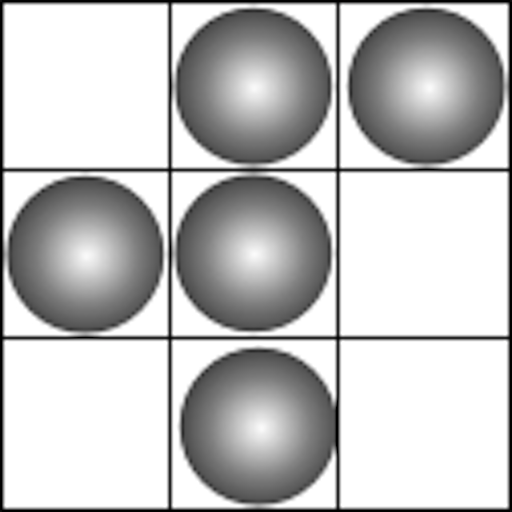
\includegraphics[width=2cm]{./r-penta512.png}
\end{center}

\begin{center}

\includegraphics[width=2cm]{./oc-logo.png}
\end{center}
\begin{center}

\includegraphics[width=2cm]{./logo-w.png}
\end{center}
\end{block}
\end{frame}
\section{パッケージを配るということ}
\label{sec:orge1f6186}
\begin{frame}[label={sec:org3b6b7ce}]{パッケージエコシステム}
\begin{itemize}
\item 作る
\item 配る
\item 使う
\end{itemize}
\end{frame}

\begin{frame}[label={sec:org39c76d1}]{パッケージを配るということ}
\begin{itemize}
\item 広く一般に向けて配る
\item 狭い範囲で限られた利用のために配る
\end{itemize}
\end{frame}

\begin{frame}[label={sec:org295148c},fragile]{広く一般に向けてpypiで配る}
 \begin{itemize}
\item PyPAツールのデフォルト
\item \texttt{tween} でアップロード
\item \texttt{pip} がダウンロードしてインストール
\end{itemize}
\end{frame}

\begin{frame}[label={sec:org75a1e5c}]{狭い範囲で限られた利用のために配る}
\begin{itemize}
\item マイクロサービスのそれぞれて使うようなライブラリ
\item 特殊なパッチをあてたローカルフレーバーライブラリ
\end{itemize}
\end{frame}

\begin{frame}[label={sec:orgc0e67d7}]{狭い範囲で配る}
\begin{itemize}
\item 社内ネットワークやVPNの中で
\item k8sやvpcの中で
\item 範囲内のIPアドレスにだけ
\item 認証をつけたい
\end{itemize}
\end{frame}

\begin{frame}[label={sec:orgebf9f5e},fragile]{httplib.server でのお手軽repository}
 \begin{itemize}
\item ダウンロードできるリンクがあればいいので \texttt{http} モジュールでサーバーを起動するだけ
\item wheelファイルのあるディレクトリで実行
\end{itemize}

\begin{verbatim}
python3 -m pip download pyramid
python3 -m http.server
\end{verbatim}

\begin{center}
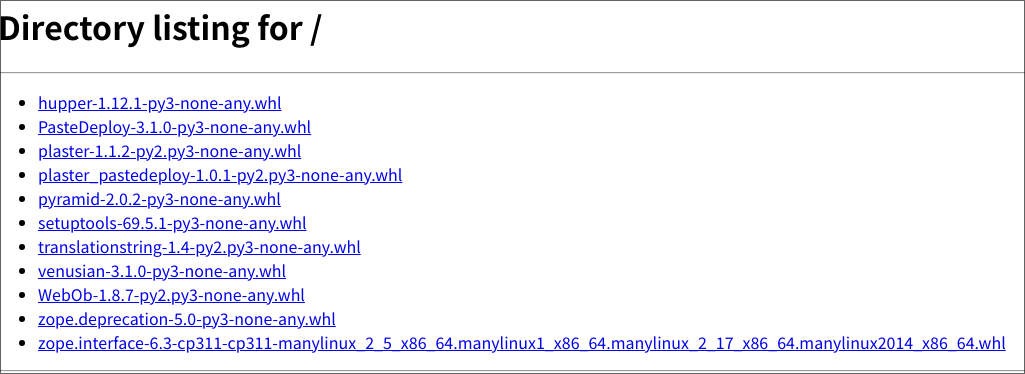
\includegraphics[width=.9\linewidth]{./http-server-simple-repository.png}
\end{center}
\end{frame}

\begin{frame}[label={sec:orge0dfa75},fragile]{URL指定でインストール}
 \begin{itemize}
\item pipはURL指定で直接インストールできる
\item 正確なファイル名を知らないといけない
\item wheelはプラットフォームなどの情報を含んでいる
\end{itemize}

\begin{verbatim}
pip install \
    http://localhost:8000/pyramid-2.0.2-py3-none-any.whl
\end{verbatim}
\end{frame}

\begin{frame}[label={sec:org1deb214},fragile]{複雑なwheelファイル名}
 \begin{itemize}
\item oh\ldots{}
\end{itemize}
\begin{verbatim}
zope.interface-6.4
-cp311
-cp311
-manylinux_2_5_x86_64.manylinux1_x86_64.manylinux_2_17_x86_64.manylinux2014_x86_64
.whl
\end{verbatim}
\end{frame}
\begin{frame}[label={sec:orgbb43150},fragile]{find-links}
 \begin{itemize}
\item \texttt{find-links} で指定した場所から探しだしてもらう
\end{itemize}
\begin{verbatim}
pip install -f http://localhost:8000 zope.interface
\end{verbatim}
\end{frame}

\begin{frame}[label={sec:org73d1d4c},fragile]{no-index}
 \begin{itemize}
\item 場合によってはpypiへの接続も制限される環境
\item 全てをお手軽repositoryから取得するなら \texttt{no-index} も使うようにしてみよう

\item \texttt{no-index} pypiなどのindexを見にいかない
\item \texttt{find-url} 指定したページからダウンロードURLをスクレーピング
\end{itemize}
\end{frame}

\begin{frame}[label={sec:orga9158fc},fragile]{indexは必要?}
 \begin{itemize}
\item pipを直接使うなら \texttt{find-url} でもいいかも?
\item メタデータを取得するのに配布物をダウンロードするという効率の悪さはある
\item \texttt{poetry source add} で使えるのは simple repository
\begin{itemize}
\item pipだと \texttt{-{}-{}index-url} で指定するものに相当
\end{itemize}
\end{itemize}
\end{frame}

\begin{frame}[label={sec:orgf58dcec},fragile]{独自のpypiを立てたい!}
 \begin{itemize}
\item PyPI自体のソースコードは公開されている
\begin{itemize}
\item \url{https://github.com/pypi/warehouse}
\item インフラ構築保守など手間もかかる
\end{itemize}
\item devpi
\begin{itemize}
\item \url{https://github.com/devpi/devpi}
\item PyPIへのプロキシやプロジェクトごとの名前空間設定など多機能
\item それなりにインフラ構築保守の手間がかかる
\end{itemize}
\item \texttt{http.server} くらいに簡単に立ち上って欲しいところ
\end{itemize}
\end{frame}

\section{パッケージを配るためのPEP}
\label{sec:orgd5ebd40}
\begin{frame}[label={sec:org24836f8}]{パッケージを配るためのPEP}
\begin{itemize}
\item \href{https://peps.python.org/pep-0458}{PEP 458 – Secure PyPI downloads with signed repository metadata}
\item \href{https://peps.python.org/pep-0480}{PEP 480 – Surviving a Compromise of PyPI: End-to-end signing of packages}
\item \href{https://peps.python.org/pep-0503/}{PEP 503 – Simple Repository API}
\item \href{https://peps.python.org/pep-0592}{PEP 592 – Adding “Yank” Support to the Simple API}
\item \href{https://peps.python.org/pep-0629}{PEP 629 – Versioning PyPI’s Simple API}
\item \href{https://peps.python.org/pep-0658}{PEP 658 – Serve Distribution Metadata in the Simple Repository API}
\item \href{https://peps.python.org/pep-0691}{PEP 691 – JSON-based Simple API for Python Package Indexes}
\item \href{https://peps.python.org/pep-0700}{PEP 700 – Additional Fields for the Simple API for Package Indexes}
\item \href{https://peps.python.org/pep-0714}{PEP 714 – Rename dist-info-metadata in the Simple API}
\end{itemize}
\end{frame}

\begin{frame}[label={sec:org71cb375}]{Simple Repository}
representation

\begin{itemize}
\item HTML PEP503
\item JSON PEP691
\end{itemize}

バージョン
\begin{itemize}
\item 1.0 PEP503/PEP691
\item 1.1 PEP700
\item PEP714 メタデータフィールドの取り扱いについての修正
\begin{itemize}
\item warehouseの実装で間違えがあったらしい
\end{itemize}
\end{itemize}
\end{frame}

\begin{frame}[label={sec:org8970cc6}]{PyPIのSimple Repository}
\begin{itemize}
\item \url{https://pypi.org/simple/} とても大きいのでアクセス注意!
\end{itemize}
\end{frame}


\begin{frame}[label={sec:orgabd614d}]{実装方針}
\begin{itemize}
\item 標準ライブラリでいこう
\begin{itemize}
\item Batteries Included!
\end{itemize}
\item 1ファイルデプロイ
\item DBなどを使わず起動するだけで使える
\end{itemize}
\end{frame}

\begin{frame}[label={sec:orgb3e3cf3}]{標準ライブラリでwebアプリケーションを書く}
\begin{itemize}
\item json
\item wsgiref
\end{itemize}
\end{frame}

\begin{frame}[label={sec:org7df21c0},fragile]{simple repositoryの機能}
 \begin{itemize}
\item 2つだけ!
\begin{itemize}
\item \texttt{/} project list
\item \texttt{/\{project\}} project detail
\end{itemize}
\end{itemize}
\end{frame}

\begin{frame}[label={sec:orga9c6a49},fragile]{project list}
 \begin{itemize}
\item ホストしているプロジェクト(ほぼパッケージの意味)を一覧で出すだけ
\item v1.0のプロジェクトに関する情報は \texttt{name} のみ
\end{itemize}
\end{frame}

\begin{frame}[label={sec:org1886530},fragile]{project list のtyping}
 \begin{verbatim}
Project = TypedDict("Project", {"name": str})
ProjectList = TypedDict(
    "ProjectList",
    {
        "meta": Meta,
        "projects": list[Project],
    },
)

\end{verbatim}
\end{frame}

\begin{frame}[label={sec:orga419fcd}]{project detail}
\begin{itemize}
\item プロジェクト(パッケージ)ごとのダウンロード可能なファイル一覧
\item ファイルのURLやパッケージメタデータなど
\end{itemize}
\end{frame}

\begin{frame}[label={sec:org67f5231},fragile]{project detailのtyping}
 \begin{verbatim}
ProjectDetail = TypedDict(
    "ProjectDetail",
    {
        "name": str,
        "files": list[ProjectFile],
        "meta": Meta,
    },
)

\end{verbatim}
\end{frame}

\begin{frame}[label={sec:org2af2007},fragile]{project fileのtyping}
 \begin{verbatim}
ProjectFile = TypedDict(
    "ProjectFile",
    {
        "filename": str,
        "url": str,
        "hashes": dict[str, str],
        "requires-python": NotRequired[str],
        "dist-info-metadata": NotRequired[str],
        "gpg-sig": NotRequired[bool],
        "yanked": NotRequired[bool],
    },
)

\end{verbatim}
\end{frame}


\begin{frame}[label={sec:org28d6772},fragile]{pypi version}
 \begin{itemize}
\item 今回はv1.0の範囲でやってみます
\end{itemize}

\begin{verbatim}
{
  "meta": {
    "api-version": "1.0"
  }
}
\end{verbatim}
\end{frame}

\begin{frame}[label={sec:orgd1423d2},fragile]{wheelファイルを探しだす}
 \begin{itemize}
\item pathlibでできちゃうね!
\item wheelファイルのファイル名は形式が決まっている
\begin{itemize}
\item PEP 491 The Wheel Binary Package Format 1.9
\item \texttt{\{distribution\}-\{version\}(-\{build tag\})?-\{python tag\}-\{abi tag\}-\{platform tag\}.whl.}
\end{itemize}
\end{itemize}
\end{frame}

\begin{frame}[label={sec:org59569c2},fragile]{metadata}
 \begin{itemize}
\item METADATAをwheelから取り出す
\item wheelはzipファイル
\item METADATAの場所は決まっている
\begin{itemize}
\item PEP 491 The Wheel Binary Package Format 1.9
\item \texttt{\{distribution\}-\{version\}.dist-info/} contains metadata.
\end{itemize}
\end{itemize}

\begin{verbatim}
def get_metadata(whl: pathlib.Path):
    parts = whl.name.split("-")
    dist_name, version = parts[0], parts[1]
    metadata_path = f"{dist_name}-{version}.dist-info/METADATA"
    with zipfile.ZipFile(whl) as zf:
        with zf.open(metadata_path) as metadata:
            return metadata.read()

\end{verbatim}
\end{frame}


\begin{frame}[label={sec:orgeed7d1a},fragile]{ダウンロード}
 \begin{itemize}
\item wheelファイルの中身をレスポンスボディにする
\item wheelのcontent-typeは特に決まってないので \texttt{application/octet-stream} にする
\item ブラウザでアクセスしたときにダウンロードになるよう \texttt{Content-Disposition} をつける
\end{itemize}
\begin{verbatim}
def get_data(self, whl: str) -> bytes:
    with self.wheels[whl]["data"].open("br") as f:
        return f.read()

\end{verbatim}
\begin{verbatim}
def __call__(self, environ, start_response) -> Iterable[bytes]:
    whl = environ["wsgiorg.routing_args"][1]["wheel_name"]
    start_response("200 OK", [("Content-type", "application/octet-stream")])
    return [self.repo.get_data(whl)]

\end{verbatim}
\end{frame}
\begin{frame}[label={sec:org6626cbe},fragile]{pipから使う}
 \begin{itemize}
\item project list呼ばれてないかも?
\end{itemize}


\begin{verbatim}
$ pip install pyramid --index-url=http://localhost:8000/
\end{verbatim}
\end{frame}

\begin{frame}[label={sec:org88f7170}]{The Update Framework}
\begin{itemize}
\item TUF
\end{itemize}
\end{frame}

\section{参考文献}
\label{sec:org97b9b4a}
\begin{frame}[label={sec:org4ed43f2}]{参考文献}
\begin{itemize}
\item PyPA Simple Repository API, \url{https://packaging.python.org/en/latest/specifications/simple-repository-api/}
\item The Update Framework, \url{https://theupdateframework.io/}
\end{itemize}
\end{frame}
\end{document}
